\subsection{Left Screen}
\subsubsection{Mock-up}
\vspace{1em}
\begin{minipage}{\linewidth}
  \begin{center}
  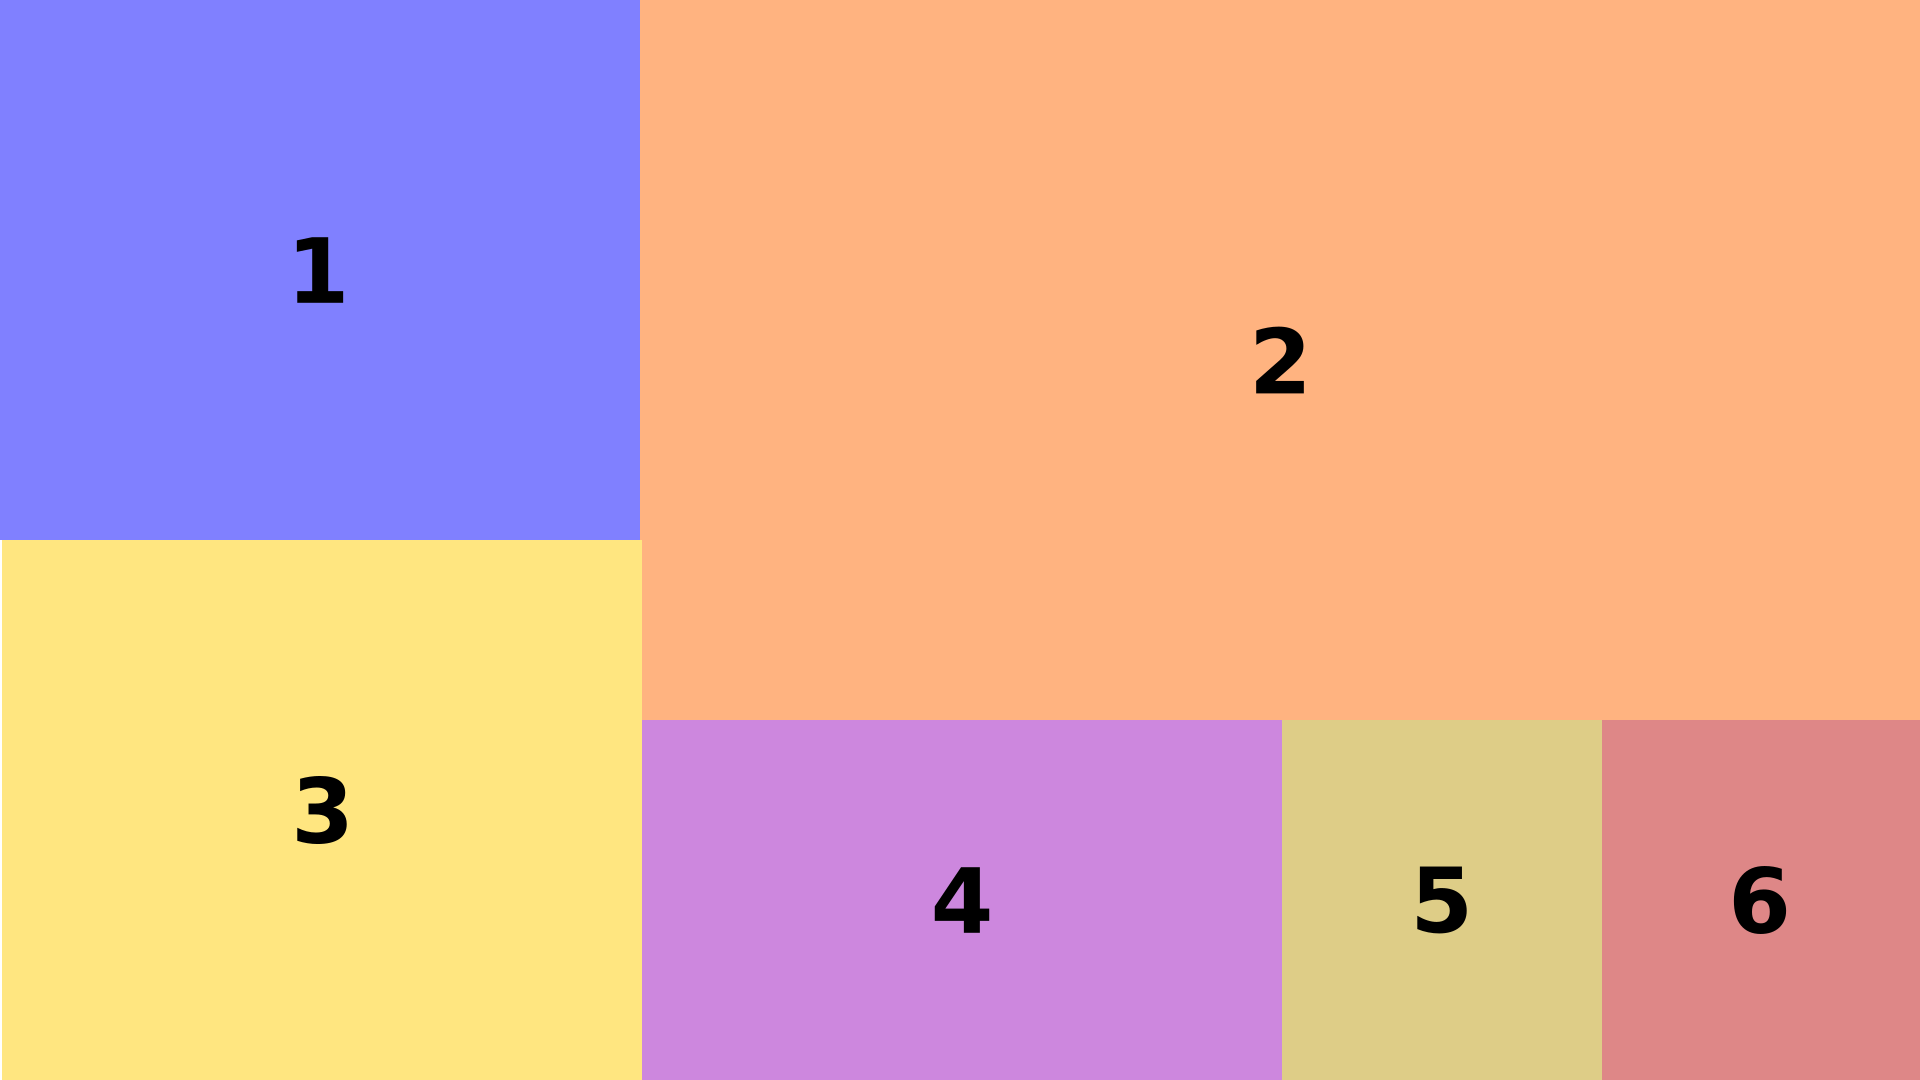
\includegraphics[width=0.75\linewidth]{left_screen_svg}
  \captionof{figure}{Left Screen Mock-up}
  \end{center}
\end{minipage}

\subsection{Zones}
\subsubsection{1: System Statuses / Sensor Readings}
This section will display all status and sensor data both from the Rover and about the ground station itself.
This includes items such as radio signal strength, GPS accuracy, and whether they Ground Station has connection to the drive joystick/s and SpaceNav mouse.

\subsubsection{2: Map Display}
The map display will display a satellite view of the competition areas with navigation and land-mark way-points, the Rover, and the Rover movement trail overlaid.

\subsubsection{3: Recording / Logging / Settings}
This section will be tabbed group that by default will show the controls for starting ROS bag recordings, but will also have a tab for live logs and a third tab for settings to adjusting items such as what map is being shown.

\subsubsection{4: Way-point Entry / Autonomy Controls}
This block will also for manual entry of GPS coordinates, as are provided by the competition at the beginning of some events.
The user will be able to chose whether the entry is being added as a navigation or landmark way-point as well as using the entry fields to edit the way-points from pre-entered points.


\subsubsection{5: Navigation Way-points Listing}
This area will list, in order, the navigation way-points that the system is currently set to follow, both for manual driving and for the autonomy portion.

\subsubsection{6: Landmark Way-points Listing}
This will list, in the order they were added, the landmark way-points that the user has entered to make important points on the competition field.

\subsection{Layout Rationale}
This display shows most of the information regarding the Rover that does not need to be viewed while the Rover is being actively driven, or while the arm is being moved.
When the software starts and is first connecting to the Rover, the user will spend some time studying system statuses, entering way-points, changing settings, and checking logs if needed.
Once they are done with these initial checks and entries, most of the rest of the control experience will take place on the right hand monitor.
In the case that the user wants to quickly glance at the map while they are driving, the map will come in to view easily as it is as close to the right hand monitor as it can be.
As the logging and setting views will hopefully not need to be viewed very often, combining them onto a tabbed GUI element helps reduce used space while still leaving them accessible when needed.


\subsection{Right Screen}
\subsubsection{Mock-up}
\vspace{1em}
\begin{minipage}{\linewidth}
  \begin{center}
  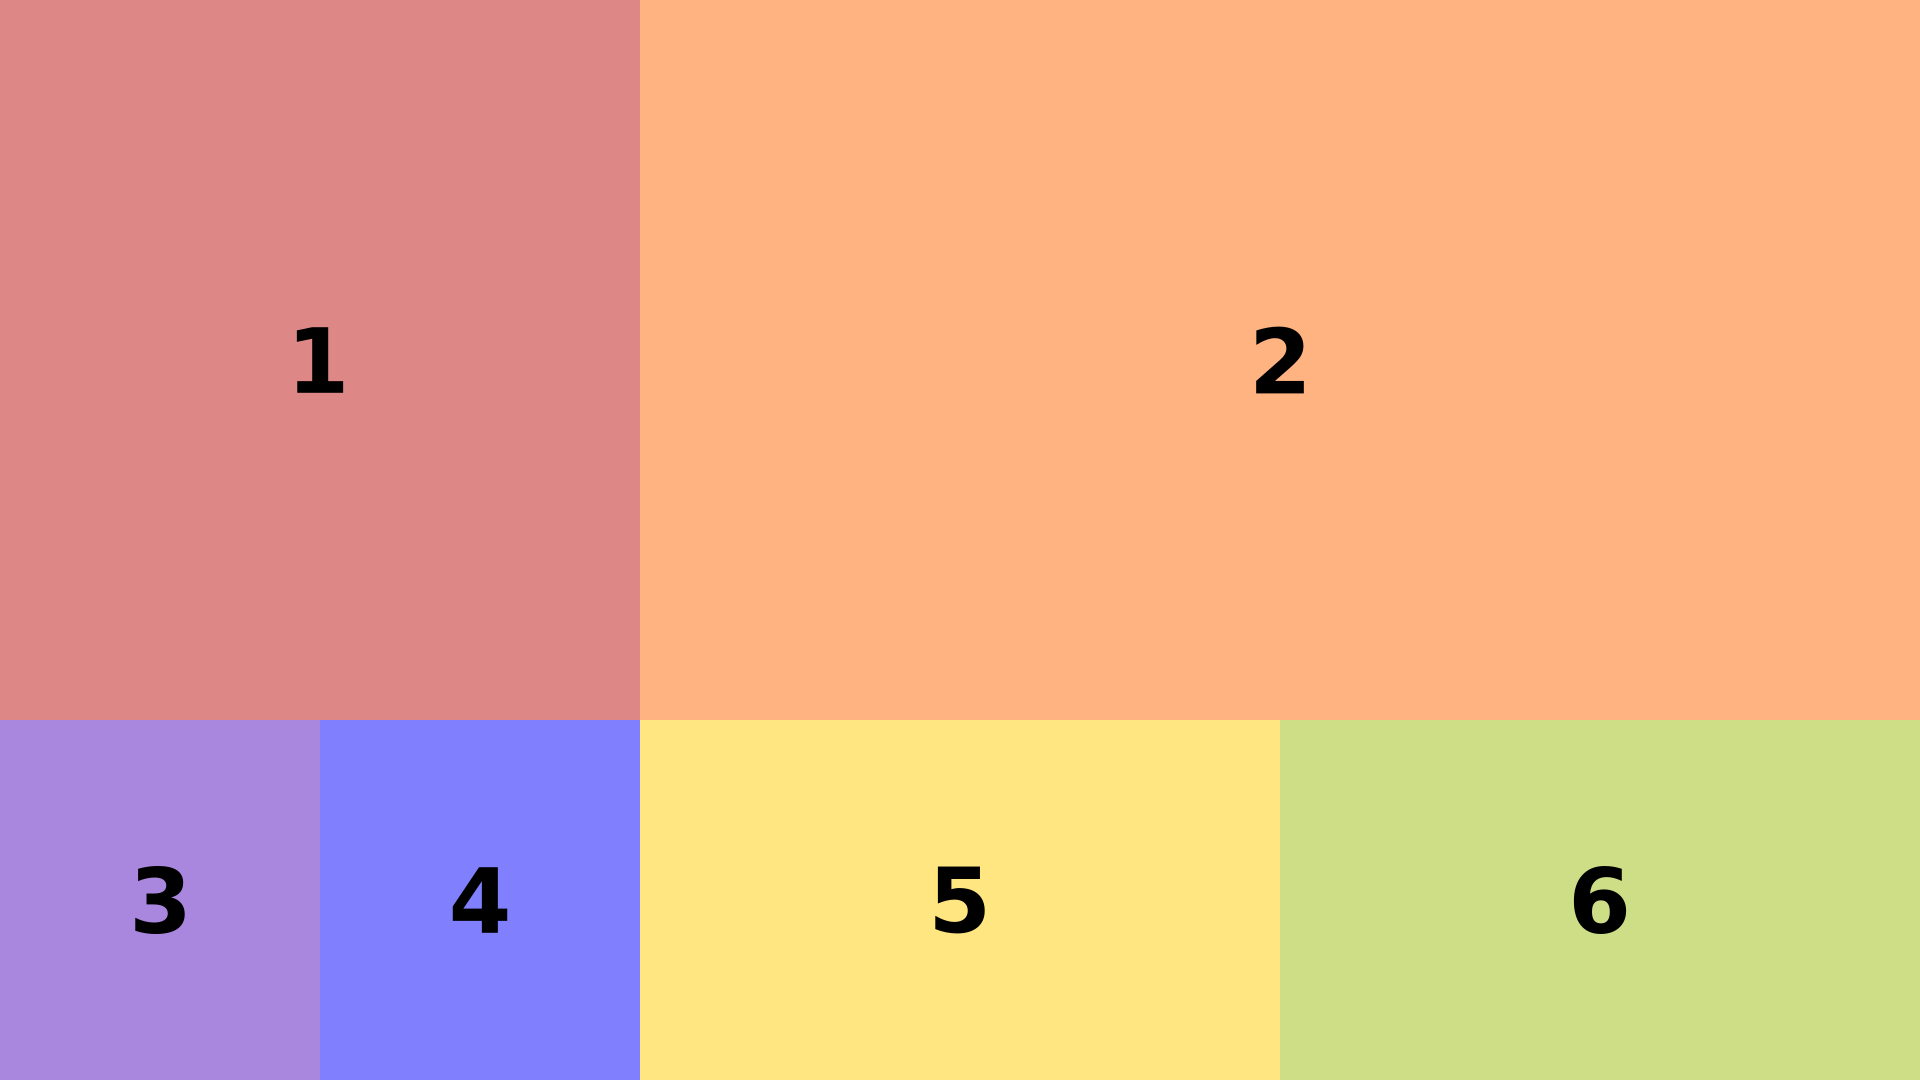
\includegraphics[width=0.75\linewidth]{right_screen_svg}
  \captionof{figure}{Right Screen Mock-up}
  \end{center}
\end{minipage}

\subsection{Zones}
\subsubsection{1: Arm Visualization}
This visualization area will show the joint positions of the Rover arm when the arm is attached.
In its simplest form, the visualization will be a simple line drawn in a reference frame, that adjusts its position as the arm is moved.
For this version, each joint would have its own visualization box.
If there is enough time, our team will attempt to integrate with RVIZ, the ROS visualization package, to show a 3D view of the arm moving.
If the RVIZ solution does not seem feasible and there is still extra time, we may alternatively try to implement a custom OpenGL view of the arm.

\subsubsection{2: Primary Video Display}
This will show the stream from the camera on the Rover is currently selected as the primary video stream.


\subsubsection{3: Heading Compass}
This heading compass will dynamically rotate to match the current heading of the Rover.
It will also mark on the compass edge the currently active way-point, making it easy for the user driving the Rover to determine which direction they need to turn to line up with a way-point marker.


\subsubsection{4: Speed and Speed Limit Display}
This area will show the current Rover speed is meters per second as is reported by the Rover GPS.
Additionally, it will also show the current speed limit of the Rover from zero to one hundred percent as has been limited by the user via the joystick throttle lever.


\subsubsection{5: Secondary Video Display}
This area will show the stream from the camera on th Rover that is currently selected as the secondary video stream.
This stream has the capability to be disabled and show a placeholder image if the team needs to save on radio bandwidth.


\subsubsection{6: Tertiary Video Display}
This area will show the stream from the camera on th Rover that is currently selected as the tertiary video stream.
This stream has the capability to be disabled and show a placeholder image if the team needs to save on radio bandwidth.


\subsection{Layout Rationale}
This screen will be showing the most commonly looked at data for the user driving the Rover.
During a normal competition, the user will start by entering way-points to drive the Rover to, and then switch to the joystick and SpaceNav mouse.
Once they start driving, the user will be heavily focused on monitoring video data to make sure they don not run the Rover into anything. 
While driving to the way-points to get to an end location, the user will be able to easily see the compass indicator, with a marker for the direction they should be heading.
After arriving at an ending way-point, the user can then seamlessly transition to moving the Rover arm (for competition challenges where this is the case) and watching the visualization update on the same screen as the video of the arm moving.
By laying out these particular elements on this screen, the user will be less likely to have to look at the left screen except when the Rover is not moving.